\chapter{Megvalósítás}

A megvalósított program osztály diagramja:

\begin{figure}[h!]
\centering
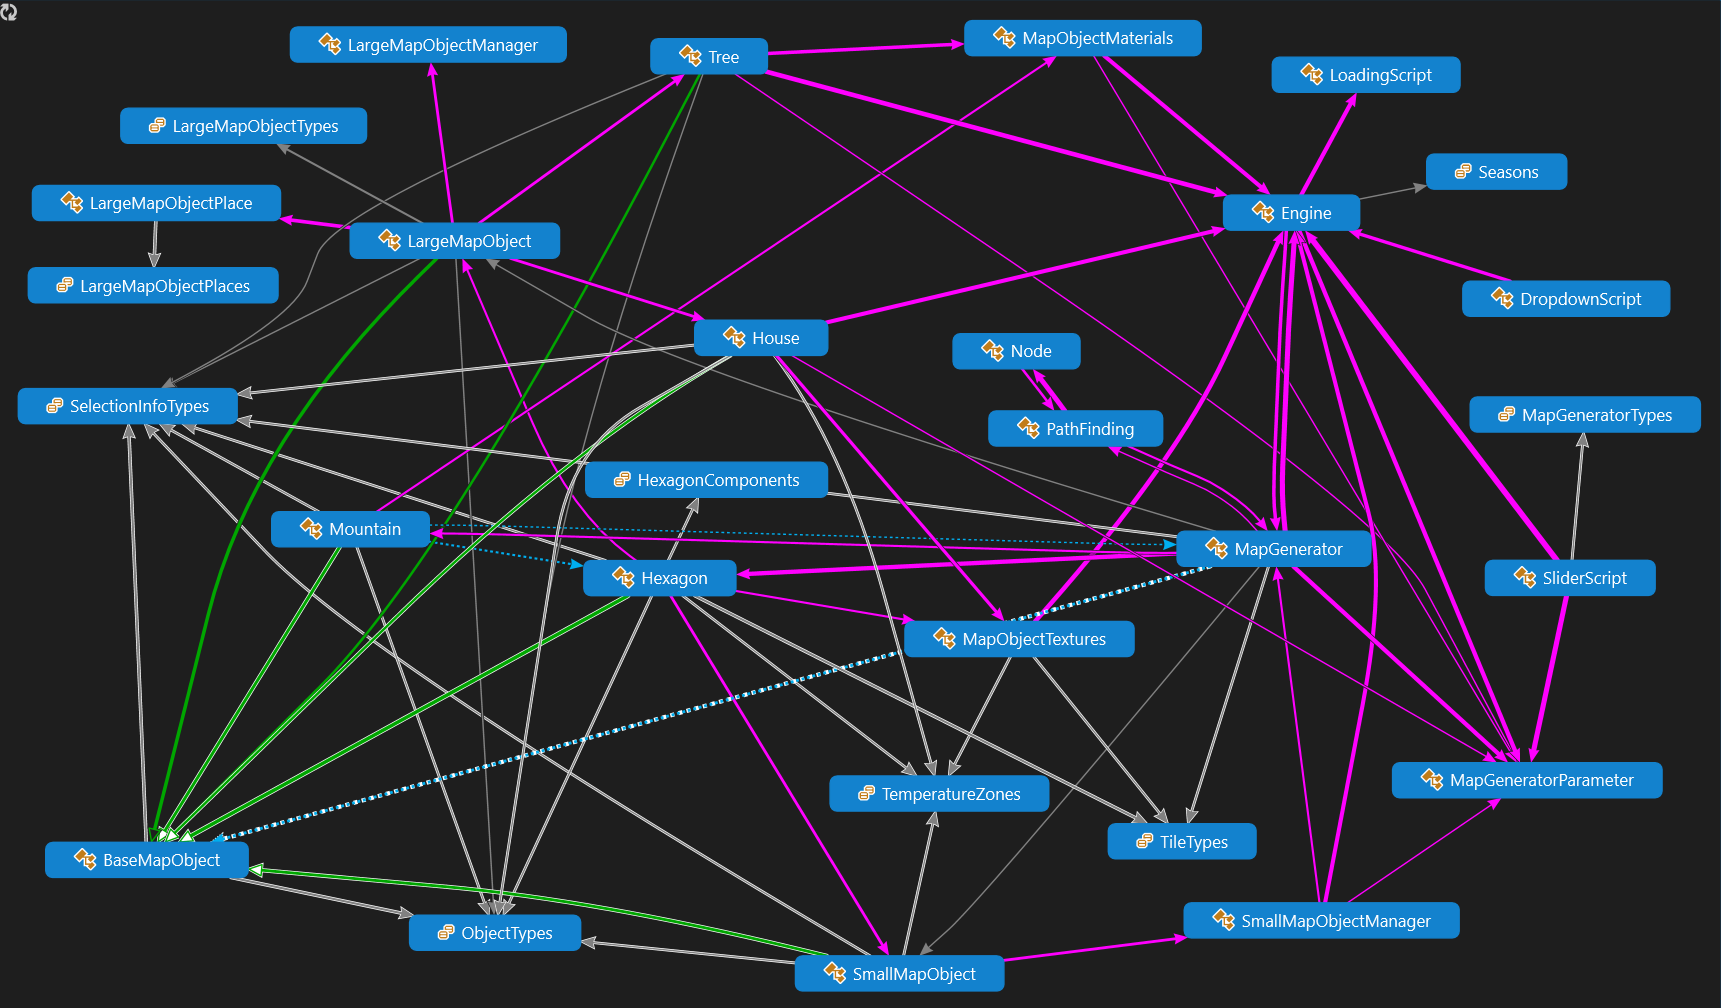
\includegraphics[scale=0.3]{kepek/szorny.png}
\caption{Az elkészült program osztály diagramja}
\label{fig:szorny}
\end{figure}

\noindent A különböző osztályokat és működésüket a következő pontokban fogom bemutatni kisebb logikailag összetartozó egységek alapján a könnyebb átláthatóság miatt. 

\section{Modellek}

\begin{figure}[h!]
\centering
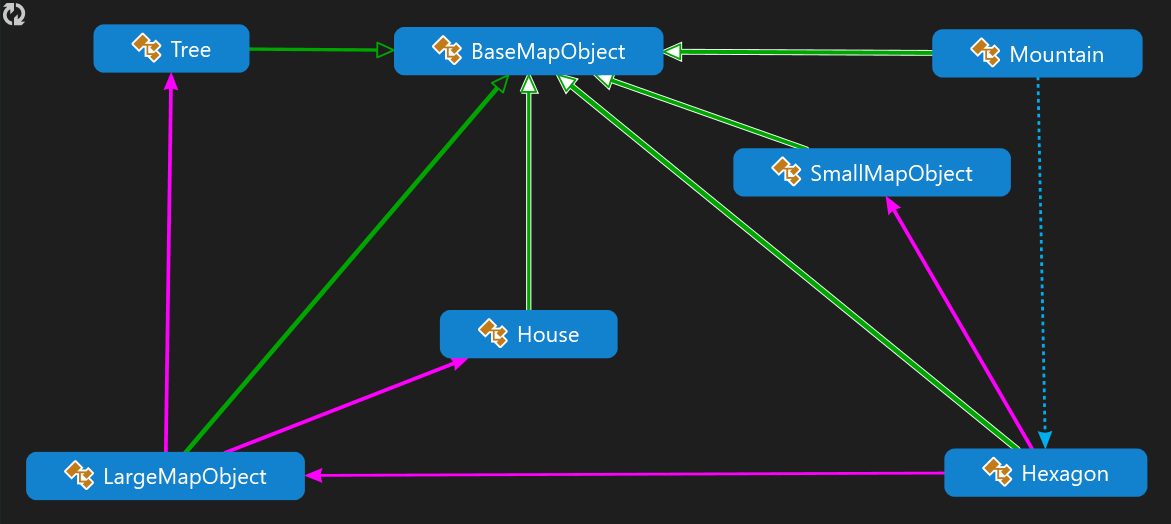
\includegraphics[scale=0.4]{kepek/modellek.png}
\caption{A programban szereplő modellek hierarchiája}
\label{fig:modellek}
\end{figure}

A BaseMapObject osztályból származik le az összes modellekhez kapcsolt osztály, ebben vannak leírva a közös tulajdonságaik a térképen szereplő objektumoknak (pozíció a térképen, milyen típusú objektum, kiválasztható vagy nem). A térképen megjelenő objektumokhoz kapcsolt osztályokat a hexagon osztály kapcsolja össze. Ez az osztály tárolja  a hexagonhoz tartozó statikus hőmérsékletet, vízszintet és amikor változás áll be az aktuális hőmérsékletben akkor meghívja a hozzá kapcsolt objektumoknak a megfelelő metódusait. A kisebb objektumok (virág, kaktusz, kő) és a nagyobb objektumok (épületek, fák) 1-1 osztályhoz (LargeMapObjectManager, SmallMapObjectManager) vannak hozzákötve, ezáltal könnyítve a kezelésüket.
\newline
\newline Minden egyes hexagon modell egy map elnevezésű üres objektum leszármazottjaként jön létre. Az összes többi modell pedig a hexagon modell leszármazottja lesz. Ezáltal könnyebben kereshetőek az objektumok a Unity API-k segítségével.
\newline
\newline A Tree osztályban egy tömbben megadható a fa modelleknek azok a részei amik a lombot alkotják. Az algoritmus pedig az környezeti viszonyoknak megfelelően módosítja (szabályozza a láthatóságát vagy az évszaknak megfelelően módosítja a színeket).
\newline
\newline Az épületek esetében is a fáknál már megismert módszert alkalmaztam arra, hogy szabályozzam a környezeti viszonyoknak a behatását az épületekre vonatkozóan.
\newline
\newline Manager osztályokat hoztam létre amikben tömbökben megadhatóak a textúrák és a materiálok, ezeket az inspector panelen lehet megadni.

\begin{figure}[h!]
\centering
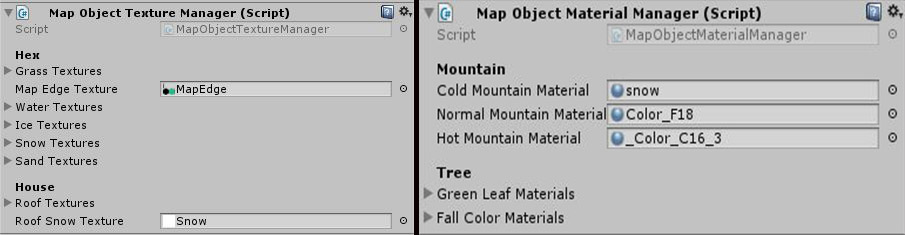
\includegraphics[scale=0.6]{kepek/Managers.jpg}
\caption{Manager osztályok állítási lehetősége az Inspector panelen}
\label{fig:Managers}
\end{figure}

\newpage
\section{UI és paraméterek szabályzása}

\begin{figure}[h!]
\centering
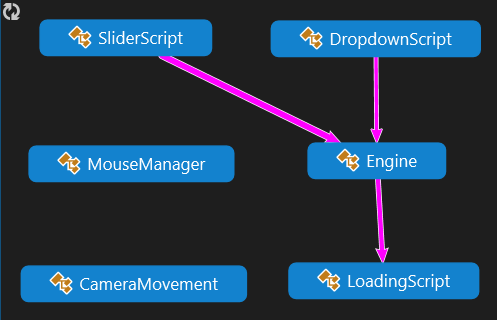
\includegraphics[scale=0.37]{kepek/UI.png}
\caption{A felhasználói felülethez kapcsolódó osztályok és az Engine kapcsolata}
\label{fig:UI}
\end{figure}

\noindent A \ref{fig:UI} ábrán bal oldalt látható a programban szereplő felhasználói felület. Az ezen található vezérlő elemek segítségével szabályozhatjuk a generálni kívánt térkép paramétereit. Minden vezérlő elemhez tartozik egy script fájl ami a játék indításakor beállítja a vezérlő elemekhez tartozó alapértéket és bizonyos esetekben a minimum, maximum vagy a további lehetséges értékeket is. Ezek az értékek az Engine osztályban vannak “beégetve”. A paraméterek aktuális értékét az Engine megfelelő metódusainak meghívásával lehet módosítani.
\newline
\newline A CameraMovement osztály felelős a kamera mozgatásért. Ennek az osztálynak a kódját a Unity store-ból szereztem be, mivel minden alapvető kritériumnak megfelelt amit terveztem és csak apróbb módosításokra volt szükségem (tengelyeken való mozgás limitálásának kiegészítése). 

\begin{figure}[h!]
\centering
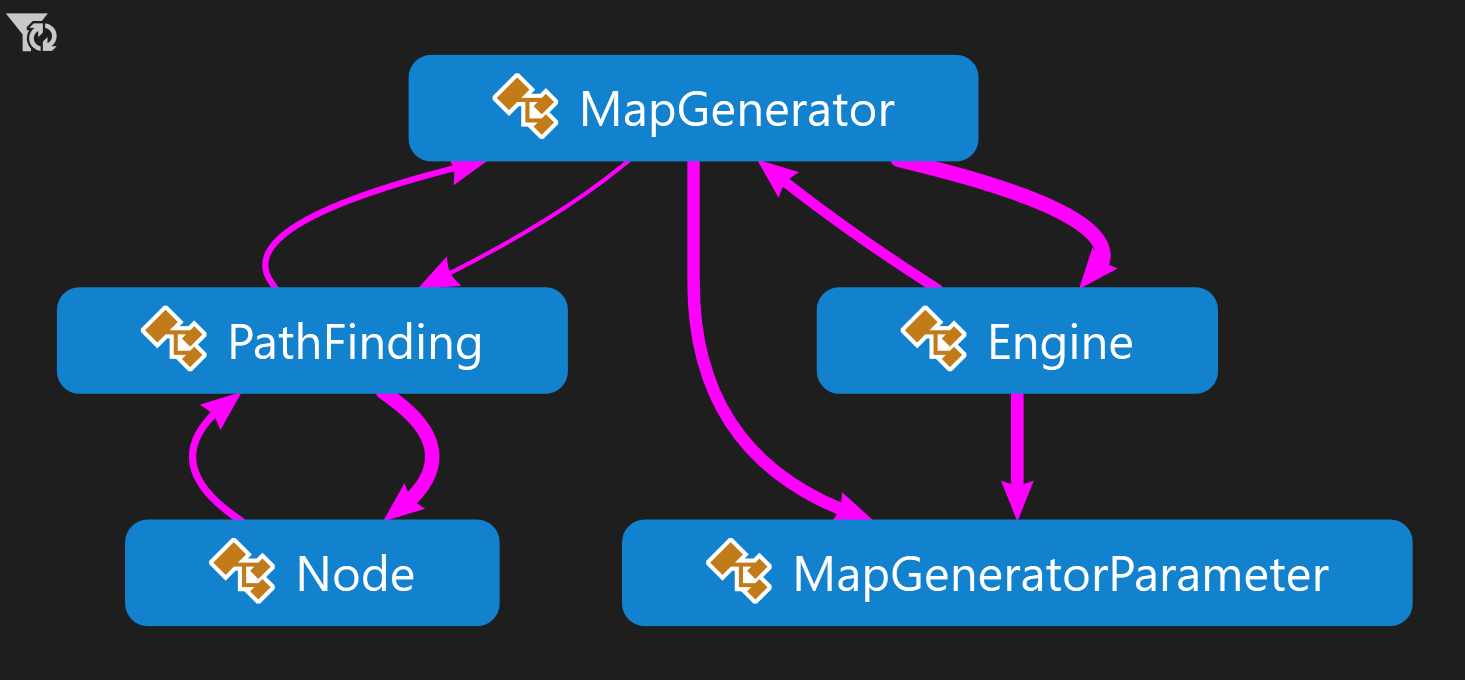
\includegraphics[scale=0.4]{kepek/generalas.png}
\caption{Generálási folyamathoz kapcsolódó főbb osztályok}
\label{fig:generalas}
\end{figure}

\noindent A MapGenerator osztály ami a generálást elvégzi, a Tervezés fejezetben már ismertetett 8 lépés alapján.

\subsection{Térkép szélének generálása:}

Jelenlegi állapotában a térképet csak valamilyen speciális textúrájú hexagonnal lehet körülhatárolni, de jövőbeli igény esetén minimális módosítások által elérhető lesz más objektumok használata is. 
\newline
\newline Algoritmus:

\begin{verbatim}
for (int x = 0; x < TérképSzélesség; x++)
{
   CsempeLétrehozása(x, 0);
   CsempeLétrehozása(x, TérképMagasság);
}
for (int y = 0; y < TérképMagasság; y++)
{
   CsempeLétrehozása(0, y);
   CsempeLétrehozása(TérképSzélesség, y);
}
\end{verbatim}

\subsection{Domborzat generálása:}

A domborzat generálása véletlenszerű pozíciókba történik.
\newline
\newline Algoritmus:

\begin{verbatim}
int DomborzatMaximálisSzáma = (TérképSzélesség * TérképMagasság
* (ParaméterÉrtéke / 100.0));

int i = 0;
while (i < DomborzatMaximálisSzáma)
{
   Vector3 pozíció= new Vector3(rnd.Next(1, TérképSzélesség - 1),
   0, rnd.Next(1, TérképMagasság - 1));

   if (Térkép[pozíció.x, pozíció.y] == null)
   {
      CsempeLétrehozásaHeggyel(pozíció);
      i++;
   }
}
\end{verbatim}

\subsection{Folyók generálása:}

A folyók generálásához A* útkereső algoritmust használtam. A nagy terjedelmű algoritmus helyett csak a pszeudokódot mutatnám be, ami alapján implementáltam ezt a részt.
\newline
\newline Algoritmus:

\begin{verbatim}
OPEN //the set of nodes to be evaluated
CLOSED //the set of nodes already evaluated
add the start node to OPEN

loop
   current = node in OPEN  with the lowest f_cost
   remove current from OPEN
   add current to CLOSED

   if current is the target node //path has been found
      return

   foreach neighbour of the current node
      if neighbour is not traversable or neighbour is in CLOSED
         skip to the next neighbour

      if new path to neighbour is shorter OR neighbour is not in OPEN
         set f_cost of neighbour
         set parent of neighbour to current
         
         if neighbour is not in OPEN
            add neighbour to OPEN
\end{verbatim}

\noindent Fontosnak tartom még megemlíteni azt, hogy az algoritmus során szükséges tárolnunk minden egyes csomópontról, hogy melyik csomópontról értük el. Amikor vizsgálunk egy csomópontot, akkor az összes szomszédját megvizsgáljuk, hogy rajta vannak-e valamelyik listán. Ha már rajta van a lezárt listán akkor tovább lépünk a következőre, viszont, ha a vizsgálandó csomópontok listáján szerepel, akkor meg kell, hogy vizsgáljuk, hogy az aktuálisan vizsgált csomópontról nem rövidebb-e az út mint a korábbi útvonal volt.

\subsection{További mezők generálása:}

Olyan mezők generálása amelyeken nem szerepel folyó vagy hegy de szerepelhetnek épületek vagy növények.
\newline
\newline Algoritmus:   

\begin{verbatim}
for (int y = 0; y < TérképMagasság; y++)
{
   for (int x = 0; x < TérképSzélesség; x++)
   {
      if (Térkép[x, y] == null)
      {
         CsempeLétrehozása(x, y);
         SzabadMezők.Hozzáad(új mező(x, y));
      }
   }
}

VárosokMaximálisSzáma= (int)(SzabadMezők.Száma 
*(ParaméterÉrtéke / 100.0));
NövényzetMaximálisSzáma= (int)(SzabadMezők.Száma 
* (ParaméterÉrtéke / 100.0));
\end{verbatim}

\noindent A szabad mezők nyilvántartásba vételére azért van szükség, hogy a generálás későbbi szakaszaiban tudjuk, hogy mennyi épületet vagy növényzetet kell generálni.

\subsection{Épületek:}
Az alábbi algoritmus véletlenszerűen kiválasztott mezőkre generál épületeket/városokat a korábban meghatározott mértékben.
\newline
\newline Algoritmus:

\begin{verbatim}
if (SzabadMezők.Száma > 0)
{
   int EddigiVárosokSzáma= 0;
    
   while ( (EddigiVárosokSzáma < VárosokMaximálisSzáma) &&
   (SzabadMezők.Száma > 0))
   {
      Vector2 index = SzabadMezők[Véletlenszám(0, SzabadMezők.Száma)];

      VárosLétrehozása(index.x, index.y);
      EddigiVárosokSzáma++;
      SzabadMezők.Eltávolítás(index);
   }
}
\end{verbatim}

\subsection{Növények:}
Ebben a pontban azt az algoritmust mutatom be, amelyik meghatározza, hogy a szabad mezők közül melyikre és milyen növényzetet generáljon.
\newline
\newline Algoritmus:

\begin{verbatim}
if (SzabadMezők.Száma > 0)
{
   int KisebbObjektumokSzáma = 0;
   int NagyobbObjektumokSzáma  = 0;

   while ( (KisebbObjektumokSzáma < NövényzetMaximálisSzáma ||
   NagyobbObjektumokSzáma  < NövényzetMaximálisSzáma ) && 
   (SzabadMezők.Száma > 0) )
   {
      Vector2 index = SzabadMezők[Véletlenszám(0, SzabadMezők.Száma)];
                
      int MeglévőNövényzet= 0;

      if (Térkép[index.x, index.y].RendelkezikKisNövényzettel)
      {
         MeglévőNövényzet += 1;
      }
      
      if (Térkép[index.x, index.y].RendelkezikNagyNövényzettel)
      {
         MeglévőNövényzet += 2;
      }

      switch (MeglévőNövényzet)
      {
         case 0:
            if (Véletlenszám(0, 1) == 0)
            {
               KisNövényzetHozzáadása(Térkép[index.x, index.y]);
               KisebbObjektumokSzáma++;
            }
            else
            {
               NagyNövényzetHozzáadása(Térkép[index.x, index.y]);
               NagyobbObjektumokSzáma ++;
            }
            break;
         case 1:
            NagyNövényzetHozzáadása(Térkép[index.x, index.y]);
            NagyobbObjektumokSzáma ++;
            break;
         case 2:
            KisNövényzetHozzáadása(Térkép[index.x, index.y]);
            KisebbObjektumokSzáma++;
            break;
         case 3:
            SzabadMezők.Eltávolítás(index);
            break;
      }
   }
}
\end{verbatim}